\section{Implementation of Algorithms}\label{sec:implementation_flow}
In this section the implementation of the main algorithm is described with use of a flowchart which illustrates the flow through code.
The main algorithm consists of three main stages, an initialization, Cov-DL for recovery of $\mathbf{A}$ and lastly M-SBL for recovery of $\mathbf{X}$. 
Considering figure \ref{fig:flow}, each stage of the algorithm is illustrated within one horizontal row of the flow diagram, furthermore the input and output are placed in their own row.    
\begin{figure}[H]
\centering
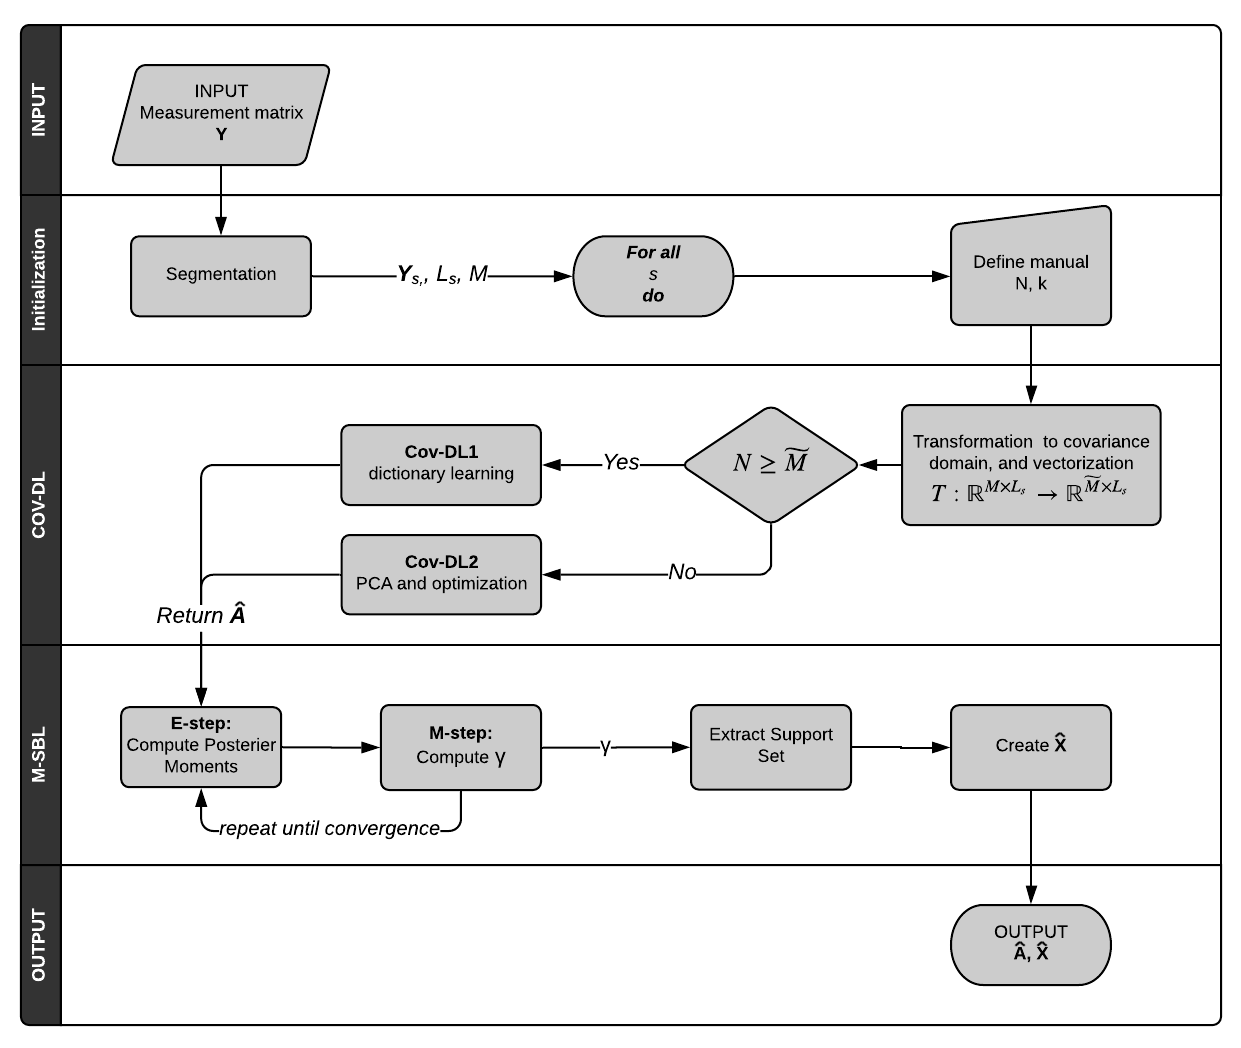
\includegraphics[scale=0.9]{figures/ch_6/baseline_flowchart.png}
\caption{Flowchart illustrating the implementation of the main algorithm.}
\label{fig:flow}
\end{figure}
The input of the main algorithm consists of the measurement matrix $\mathbf{Y} \in \mathbb{R}^{M \times L}$, along with the corresponding sample frequency $f$. 
Within the initialization stage the measurement matrix $\mathbf{Y}$ go through segmentation as described in subsection \ref{seg_segmentation}. 
The length of the segments is predefined by a time interval $t$ in seconds such that $L_{s} = tf$. 
Each segment $s$ is now specified by the measurement matrix $\mathbf{Y}_s \in \mathbb{R}^{M \times L_{s}}$.
After the segmentation a loop is constructed such that for every segments $s$ the remaining two stages, Cov-DL and M-SBL, of the main algorithm are performed. 
For each segment $s$, $N$ and $k$ are manually defined. 
This definition is either known in advance from the data or in the case of real EEG measurements they are unknown and a qualified guess must be made.
With one segment and corresponding specifications of the expected number of active sources, the second stage of the algorithm are initialised, recovery of $\mathbf{A}$.
The implementation of Cov-DL stage follows algorithm \ref{alg:Cov1} from section \ref{seg:alg_cov} closely thus only the main steps are illustrated on the flow diagram.
First the measurement matrix $\mathbf{Y}_s$ for all segments are transformed to the covariance domain and then vectorized, resulting in an extension of the dimensionality of $\mathbf{Y}$ from $M$ to $\widetilde{M} = \frac{M(M+1)}{2}$.
Next, the estimation of $\mathbf{A}$ is performed from either Cov-DL1 or Cov-DL2 depending on the relation between $\widetilde{M}$ and $N$, as described respectively in section \ref{sec:cov1} and \ref{sec:over_det}.
The estimate $\hat{\mathbf{A}}$ serves as the input to the next stage, M-SBL for recovering of $\mathbf{X}$, along with the measurement matrix $\mathbf{Y}_s$. 
The last stage of the main algorithm consists of the iterative EM algorithm for maximizing the marginal likelihood \eqref{eq:likelihood} with respect to $\boldsymbol{\gamma}$, which is the hyperparameter from which $\mathbf{X}$ can be determined as described in section \ref{seg:M_sblalg}. 
Lastly, the output of the main algorithm $\hat{\mathbf{X}}$ and $\hat{\mathbf{A}}$ is illustrated on the flowchart.

\subsection{Coding Practice}
The implementation of the main algorithm is performed in Python 3.6. The software and guide to run the scripts are available through appendix \ref{App:code}.

The practical implementation process is based on module development. 
The established model and the three stages of the main algorithm make the system design. 
For each stage the necessary tasks are identified and divided into smaller modules. 
For each module the task is specified, and the algorithms are established and implemented. 
This is followed by a test of the module and possible modifications until the task is performed without error. 
Due to the time limitation of this project, the software was developed along side the dynamic research process. 
Thus, the specifications to some modules have been redefined and hence the modification process are repeated. 
Finally, the modules are united into one stage for which tests are performed, and lastly all the stages are united to the resulting main algorithm.

The software is based on functions, for example one module is specified by one function, for which docstrings is used, following NumPy docstring format\footnote{\url{https://numpydoc.readthedocs.io/en/latest/}} allowing insight into the structure and thoughts behind the different software elements.

For each of the stages, Cov-DL and M-SBL, verification and performance tests will be performed and described later in this chapter, followed by testing phase of the main algorithm. 

